\documentclass[border=5pt]{standalone}
\usepackage[utf8]{inputenc}
\usepackage{amssymb}
\usepackage{amsmath}
\usepackage{tikz}
\usetikzlibrary{automata,arrows,positioning,calc}

\tikzset{auto shift/.style={auto=right,->,
to path={ let \p1=(\tikztostart),\p2=(\tikztotarget),
\n1={atan2(\y2-\y1,\x2-\x1)},\n2={\n1+180}
in ($(\tikztostart.{\n1})!1mm!270:(\tikztotarget.{\n2})$) -- 
($(\tikztotarget.{\n2})!1mm!90:(\tikztostart.{\n1})$) \tikztonodes}}}

\begin{document}
\nopagecolor
\begin{tabular}{c}
    Example 1 \\ \\
    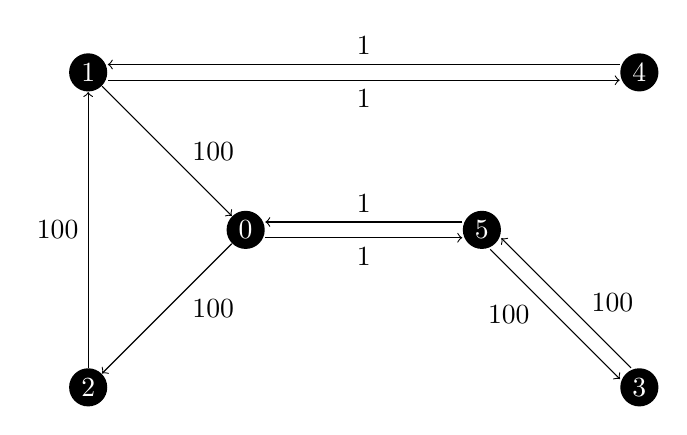
\begin{tikzpicture}
        \node[circle, inner sep=2pt, fill] (0) at (-1.5, 0) {\color{white} 0};
        \node[circle, inner sep=2pt, fill] (1) at (-3.5, 2) {\color{white} 1};
        \node[circle, inner sep=2pt, fill] (2) at (-3.5, -2) {\color{white} 2};
        \node[circle, inner sep=2pt, fill] (3) at (3.5, -2) {\color{white} 3};
        \node[circle, inner sep=2pt, fill] (4) at (3.5, 2) {\color{white} 4};
        \node[circle, inner sep=2pt, fill] (5) at (1.5, 0) {\color{white} 5};
        
        \draw (0) edge[auto shift] node[below]{1} (5)
              (5) edge[auto shift] node[above]{1} (0)
    
              (5) edge[auto shift] node[left, xshift=-0.2cm]{100} (3)
              (3) edge[auto shift] node[right, xshift=0.2cm]{100} (5)
    
              (1) edge[auto shift] node[below]{1} (4)
              (4) edge[auto shift] node[above]{1} (1)
    
              (0) edge[->] node[right, xshift=0.2cm]{100} (2)
              (1) edge[->] node[right, xshift=0.2cm]{100} (0)
              (2) edge[->] node[left]{100} (1)
              ;
    \end{tikzpicture} \\ \\
    Example 2 \\ \\
    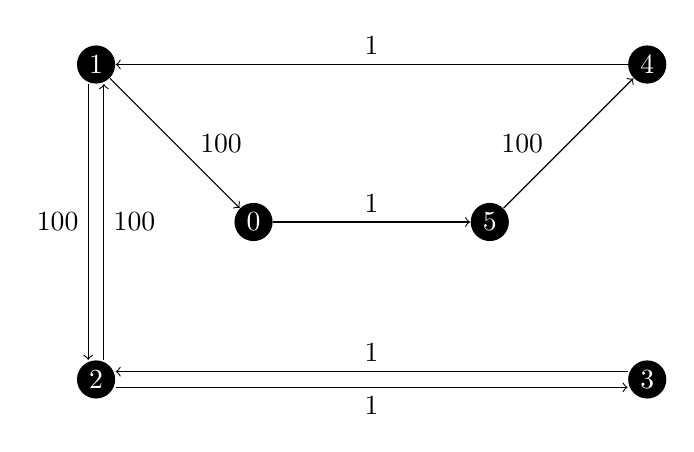
\begin{tikzpicture}
        \node[circle, inner sep=2pt, fill] (0) at (-1.5, 0) {\color{white} 0};
        \node[circle, inner sep=2pt, fill] (1) at (-3.5, 2) {\color{white} 1};
        \node[circle, inner sep=2pt, fill] (2) at (-3.5, -2) {\color{white} 2};
        \node[circle, inner sep=2pt, fill] (3) at (3.5, -2) {\color{white} 3};
        \node[circle, inner sep=2pt, fill] (4) at (3.5, 2) {\color{white} 4};
        \node[circle, inner sep=2pt, fill] (5) at (1.5, 0) {\color{white} 5};

        \draw (2) edge[auto shift] node[below]{1} (3)
              (3) edge[auto shift] node[above] {1} (2)
              
              (1) edge[auto shift] node[left]{100} (2)
              (2) edge[auto shift] node[right]{100} (1)
              
              (1) edge[->] node[right, xshift=0.2cm]{100} (0)
              (0) edge[->] node[above]{1} (5)
              (5) edge[->] node[left, xshift=-0.2cm]{100} (4)
              (4) edge[->] node[above]{1} (1)
              ;
    \end{tikzpicture} \\ \\
    Example 3 \\ \\
    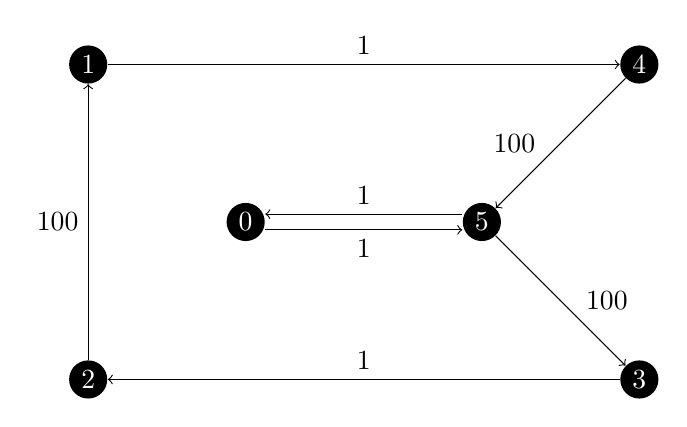
\begin{tikzpicture}
        \node[circle, inner sep=2pt, fill] (0) at (-1.5, 0) {\color{white} 0};
        \node[circle, inner sep=2pt, fill] (1) at (-3.5, 2) {\color{white} 1};
        \node[circle, inner sep=2pt, fill] (2) at (-3.5, -2) {\color{white} 2};
        \node[circle, inner sep=2pt, fill] (3) at (3.5, -2) {\color{white} 3};
        \node[circle, inner sep=2pt, fill] (4) at (3.5, 2) {\color{white} 4};
        \node[circle, inner sep=2pt, fill] (5) at (1.5, 0) {\color{white} 5};

        \draw (0) edge[auto shift] node[below]{1} (5)
              (5) edge[auto shift] node[above]{1} (0)
              
              (5) edge[->] node[right, xshift=0.2cm]{100} (3)
              (3) edge[->] node[above]{1} (2)
              (2) edge[->] node[left]{100} (1)
              (1) edge[->] node[above]{1} (4)
              (4) edge[->] node[left, xshift=-0.2cm]{100} (5)
              ;
    \end{tikzpicture} \\
\end{tabular}
\end{document}